\documentclass[tikz,border=10pt]{standalone}
\usetikzlibrary{shapes.multipart, positioning, arrows.meta, calc, backgrounds}

\begin{document}
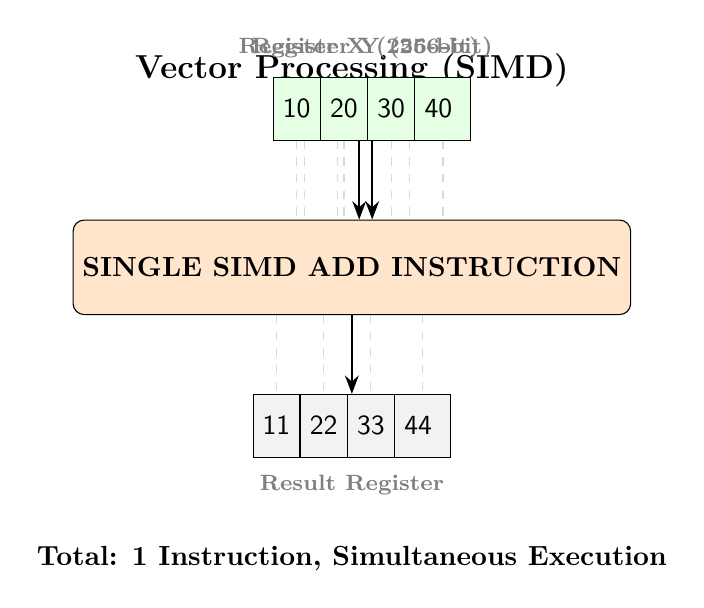
\begin{tikzpicture}[
    node distance=1.5cm,
    font=\sffamily,
    % Styles
    vector_green/.style={
        draw,
        rectangle split,
        rectangle split parts=4,
        rectangle split horizontal,
        minimum height=0.8cm,
        align=center,
        fill=green!10,
        minimum width=4cm
    },
      vector_gray/.style={
        draw,
        rectangle split,
        rectangle split parts=4,
        rectangle split horizontal,
        minimum height=0.8cm,
        align=center,
        fill=gray!10,
        minimum width=4cm
    },
    simd_op/.style={
        draw,
        rounded corners,
        fill=orange!20,
        minimum width=6cm,
        minimum height=1.2cm,
        align=center,
        font=\bfseries
    },
    arrow/.style={->, >=Stealth, thick, rounded corners},
    reg_label/.style={font=\footnotesize\bfseries, color=gray}
]

    % --- Title ---
    \node[font=\large\bfseries] at (0, 2.5) {Vector Processing (SIMD)};

    % --- CENTER OPERATION ---
    \node[simd_op] (alu) at (0, 0) {SINGLE SIMD ADD INSTRUCTION};

    % --- INPUT VECTORS ---
    % Vector X (Top Left)
    \node[vector_green, above left=1cm and -1cm of alu.north] (vx) {
        \nodepart{one} 1 \nodepart{two} 2 \nodepart{three} 3 \nodepart{four} 4
    };
    \node[reg_label, above=0.1cm of vx] {Register X (256-bit)};

    % Vector Y (Top Right)
    \node[vector_green, above right=1cm and -1cm of alu.north] (vy) {
        \nodepart{one} 10 \nodepart{two} 20 \nodepart{three} 30 \nodepart{four} 40
    };
    \node[reg_label, above=0.1cm of vy] {Register Y (256-bit)};


    % --- RESULT VECTOR ---
    \node[vector_gray, below=1cm of alu] (vres) {
        \nodepart{one} 11 \nodepart{two} 22 \nodepart{three} 33 \nodepart{four} 44
    };
    \node[reg_label, below=0.1cm of vres] {Result Register};

    % --- ARROWS ---
    \draw[arrow] (vx.south) -- (alu.north -| vx.south);
    \draw[arrow] (vy.south) -- (alu.north -| vy.south);
    \draw[arrow] (alu.south) -- (vres.north);


    % --- VISUAL GUIDE FOR PARALLELISM ---
    % Hardcoded to avoid loop parsing errors
    \begin{scope}[on background layer]
        % Element 1
        \draw[dashed, gray!30, thin] (vx.one south) -- (vx.one south |- alu.north);
        \draw[dashed, gray!30, thin] (vy.one south) -- (vy.one south |- alu.north);
        \draw[dashed, gray!30, thin] (alu.south -| vres.one north) -- (vres.one north);

        % Element 2
        \draw[dashed, gray!30, thin] (vx.two south) -- (vx.two south |- alu.north);
        \draw[dashed, gray!30, thin] (vy.two south) -- (vy.two south |- alu.north);
        \draw[dashed, gray!30, thin] (alu.south -| vres.two north) -- (vres.two north);

        % Element 3
        \draw[dashed, gray!30, thin] (vx.three south) -- (vx.three south |- alu.north);
        \draw[dashed, gray!30, thin] (vy.three south) -- (vy.three south |- alu.north);
        \draw[dashed, gray!30, thin] (alu.south -| vres.three north) -- (vres.three north);

        % Element 4
        \draw[dashed, gray!30, thin] (vx.four south) -- (vx.four south |- alu.north);
        \draw[dashed, gray!30, thin] (vy.four south) -- (vy.four south |- alu.north);
        \draw[dashed, gray!30, thin] (alu.south -| vres.four north) -- (vres.four north);
    \end{scope}

    % Annotation
    \node[below=1cm of vres, font=\bfseries] {\textbf{Total:} 1 Instruction, Simultaneous Execution};

\end{tikzpicture}
\end{document}
